\chapter{méthodes (MIC 2010)}

J'ai utilisé la base de donnée présentée dans la partie\ref{lab:bdd} pour évaluer les performances des techniques de correction du mouvement respiratoire présentés dans le chapitre \ref{lab:corrMvt}. 

Les techniques de correction du mouvement implémentées sont les suivantes :

\begin{enumerate}
 \item Correction pendant la reconstruction par modification de la matrice système (voir section \ref{lab:corrMatSyst})
 \item Correction post-reconstruction par recalage des images prises à différents instants du cycle (voir section \ref{lab:corrPostRecon})
\end{enumerate}

Elles sont comparées avec les images non Corrigées et des images statiques (qui représentent une correction parfaite).

Dans le cas présent, l'objectif est de d'évaluer les performances des techniques de correction du mouvement sur la détection des lésions de faible contraste/faible diamètre. Pour cela, je vais comparer les performances d'un système de détection automatique sur les différents types d'images.

\section{Système CAD}

Le système CAD utilise des informations fréquentielles obtenue par décomposition des images en ondelettes Biorthogonale 4.4. Ces données sont utilisées par le système de classification basé sur un SVM travaillant voxel par voxel. Une étape de réduction des faux positifs est ajoutée par la suite.

\subsection{Classifications}

\begin{enumerate}
 \item Décomposition des images en ondelettes : Pour chaque voxel de l'image d'origine, on obtient entre 8 et 32 coefficients, qui correspondent au vecteur de caractéristiques utilisés par le classifieur
 \item Extraction de la base d'apprentissage : Les coefficients des centres de toutes les tumeurs sont extraites des volumes décomposés, et vont former la base d'apprentissage H1 (positifs). Un certain nombre de voxels sont tirés aléatoirement dans chaque images et leur coefficients sont ajoutés à la base H0 (négatifs).
 \item Apprentissage : Le classifieur SVM est entraîné sur cette base d'apprentissage pour générer le modèle qui sera utilisé pour le test.
 \item Tests : Le SVM entraîné est utilisé pour classer chaque voxel contenu dans les organes à évaluer (poumon et foie).
 \item Réduction des Faux-positifs : Les points sont agrégés en composantes connexes (connexité 27 en 3 dimensions). Chaque agrégat est testé pour déterminer si il doit être considéré comme un faux positif ou un vrai positif.
\end{enumerate}

\section{Optimisation des paramètres du classifieur}
\label{lab:optim}

Les différentes étapes de l'évaluation des performances nécessitent la fixation d'un grand nombre de paramètres. Tous ceux qui correspondent à l'étape de classification sont adaptés à la modalité à évaluer, tandis que ceux relatifs au processus dans son ensemble sont fixés une seule fois.

\subsection{Paramètres à optimiser pour chaque modalité}

\begin{description}
 \item[C] Le terme de pénalisation des exemples mal classés par le classifieur
 \item[gamma] La largeur de bande du RBF du noyau du classifieur
 \item[j] Le niveau de décomposition des images 
\end{description}

J'ai effectué une recherche exhaustive par grille avec les paramètres suivants :

\begin{description}
 \item [C] de 1 à 10000 en 15 pas logarithmique
 \item [gamma] de 0.0001 à 1 en 15 pas logarithmique
 \item [j] de 1 à 4, soit de 8 à 32 caractéristiques
\end{description}

L'optimisation a été réalisée à l'aide du logiciel rapid-i~\cite{mierswa2006} pour chaque modalité. Les indicateur de performance (Sensibilité, Spécificité, Précision) sont obtenues en réalisant une cross-validation à 5 étapes sur l'ensemble de la base d'apprentissage. Le triplet de paramètre retenu est celui qui maximise la sensibilité.

J'ai joint pour chaque modalité le front de pareto positionnant chaque triplet dans un espace à deux dimensions (`Sensibilité', 'Spécificité'). Cela permet de vérifier que le critère choisit (maximisation de la sensibilité) ne se fait pas trop au détriment de la spécificité.

\subsection{Paramètres globaux}

Trois paramètres sont appliqués sur toutes les données de la même manière :
\begin{description}
 \item[Normalisation :] Les données sont normalisées de manière à ce que la moyenne et l'\emph{écart}-type de chaque caractéristique soit de 1 ($(\mu, \sigma)=(1,1)$) (\emph{moyenne}), ou alors pour que l'ensemble des valeurs soit comprises entre -1 et +1 (\emph{écart}).
 \item[Nombre de points de la base d'apprentissage :] Le nombre de points extraits de chaque image pour alimenter la base d'exemples normaux peut avoir une influence sur les résultats. Trois valeurs sont testées. 100 pts/im. (soit 1500 pts. négatifs), 200 pts/im. (soit 3000 pts. négatifs) et 1000 pts/im. (soit 15000 pts. négatifs).
 \item[positions des points extraits :] Les points normaux extraits de la base d'image peuvent être extraits de tout le volume de l'organe hors tumeurs, ou bien extraits préférentiellement des 
\end{description}

Le but de la normalisation est d'homogénéiser les plages de valeurs des différentes caractéristiques pour faciliter le travail du classifieur, dont les paramètres C et gamma dépendent de la distance entre les points et ne permettent pas de gérer des différences trop importantes d'étendues dans les caractéristiques. La première méthode de normalisation a l'avantage d'être relativement peu sensible aux valeurs extrêmes, contrairement à la seconde.

Le nombre de point de la base d'apprentissage détermine directement la qualité de l'apprentissage. Le nombre de caractéristique est de $8 \times j$, avec $j$ le niveau de décomposition des images. Il n'existe pas de règle définitive pour déterminer le nombre d'exemples nécessaire en fonction du nombre de caractéristiques, mais les SVM sont relativement bon pou éviter le sur-apprentissage. Dans notre cas, il vaudrait donc mieux avoir plus de données. Cependant, le nombre de points notés ``tumeurs'' est limité par le nombre de tumeurs présentes dans la base d'apprentissage (173 tumeurs pour le poumon, 106 pour le foie). Dans ce cas, il y a un risque de déséquilibre de la base d'apprentissage, qui devrait idéalement avoir le même nombre d'exemples ``tumeur'' que ``normales``. Des techniques de correction existent pour les SVM pour contrebalancer ces déséquilibres en indiquant un paramètre C différent pour chaque classe, mais les tests que j'ai réalisé ne montrent pas d'améliorations significatives des performances.

Les points normaux extraits des images pour alimenter la base vont avoir une influence directe sur la qualité des résultats. Idéalement ils devraient être représentatif de l'ensemble des cas rencontrés dans la base de tests, mais les bordures de certains organes peuvent ressembler à des tumeurs, et rendre l'estimation de la surface de séparation plus difficile. J'ai donc voulu évaluer la performance du CAD sur une base dépourvue des données ambigues. Pour cela j'ai réalisé une érosion de 2 voxels sur les le masque des volumes à extraire.

\section{Réduction des faux positifs}

\subsection{Création des agrégats}

Les résultats de la classification des images forment des cartes de score, qui sont 
\subsection{Critère basés sur l'intersection}

Les points classés positifs sont regroupés en amas de points connexes (connexité 27 en 3D). Il y a un ensemble de règles qui vont déterminer si un amas intersectant une lésions représente un vrai positif. Soit $L$ l'ensemble des points de la lésion, $A$ les points correspondant à l'amas candidat.

\begin{description}
 \item[$card( L \cap A ) > \alpha \times card( L )$] avec $\alpha$ fixé à 0.05 qui fixe la proportion minimale de la tumeur qui doit être présente dans l'amas. Elle permet d'éviter les amas qui intersecteraient la tumeur par accident.
 \item[$card( L \cap A ) > \beta \times card( A )$]  avec $\beta$ fixé à 0.20 limite l'étendue de l'amas en dehors de la tumeur.
\end{description}


\chapter{Analyse des résultats}


\section{Tests de différents paramètres}

Tests de 3 types de paramètres : 


\begin{figure}[h!]
\label{fig:paretoParams1}
\begin{center}
 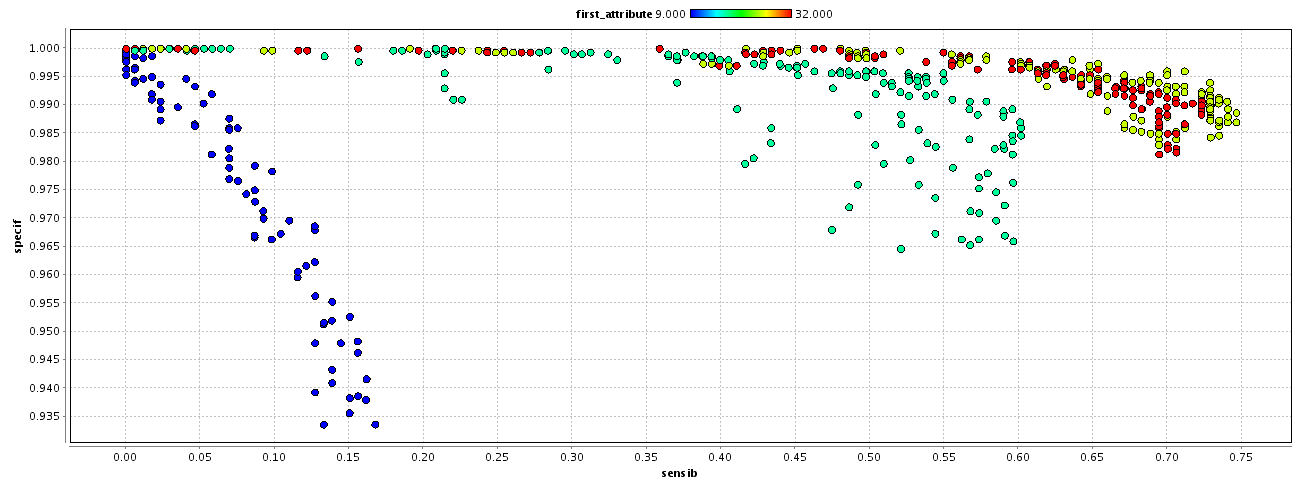
\includegraphics[width=14cm]{images/pareto_param_200.png}

{\small a) Base Témoin}
\vspace{0.5cm}

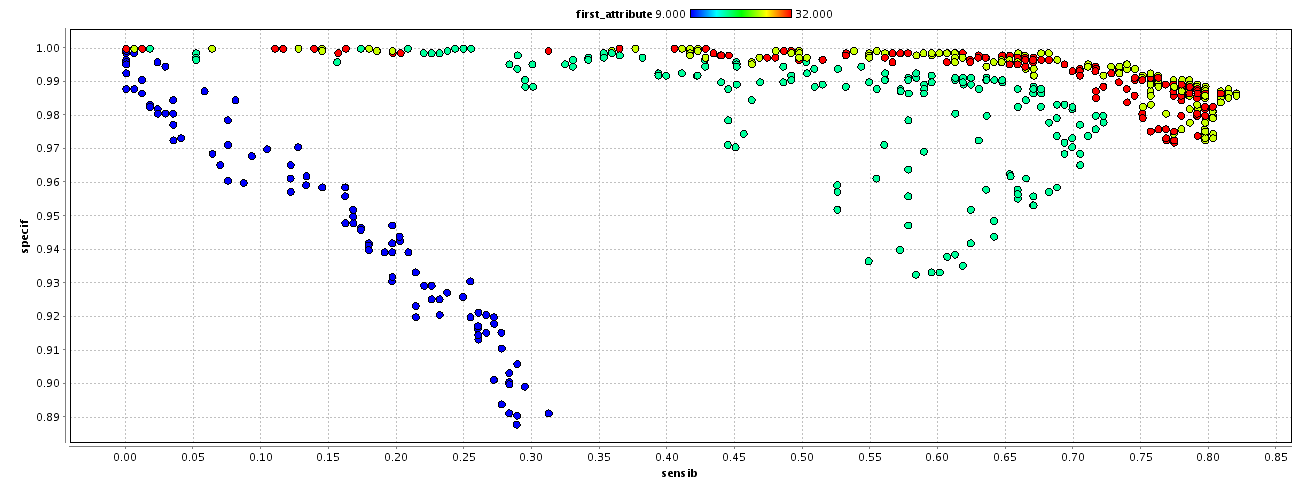
\includegraphics[width=14cm]{images/pareto_param_100.png}

{\small b) Base appauvrie}


 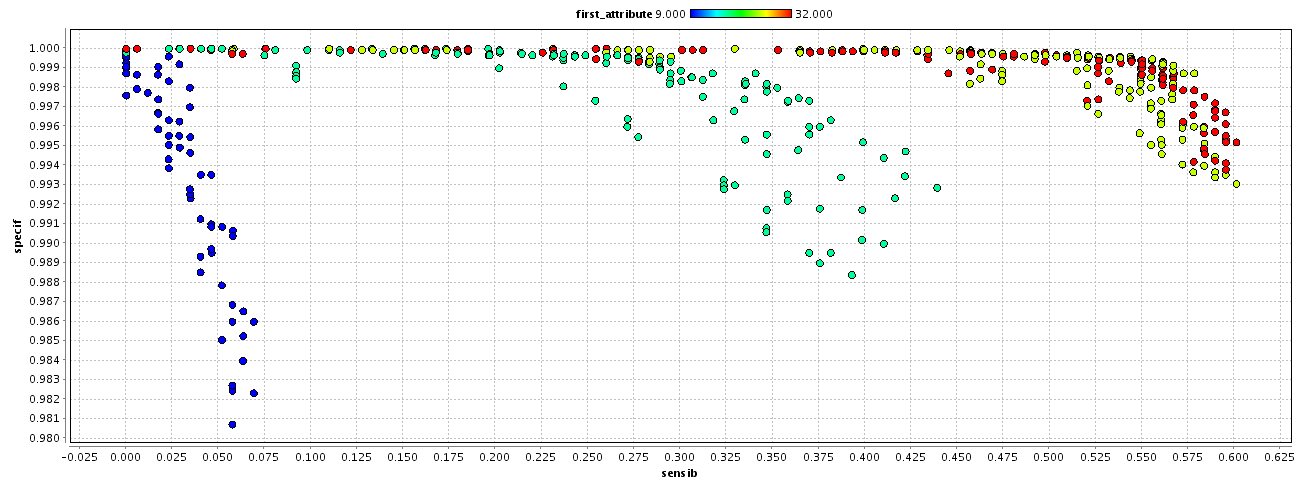
\includegraphics[width=14cm]{images/pareto_param_1000.png}
 
{\small c) Base enrichie}



\end{center}
 \caption{Fronts de pareto des résultats de la recherche des meilleurs paramètres du classifieur (1/2). Pour chaque triplet de paramètres (C, $\gamma$, j), la sensibilité et la spécificité sont reportées sur le graphique. Le code couleur correspond à la valeur de j. En a), la base témoin, avec 200 points négatifs par image et une normalisation \emph{moyenne}, en b) la base appauvrie avec 100 points négatifs par image et une normalisation \emph{moyenne}, et en c) la base enrichie avec 1000 points négatifs par image et une normalisation \emph{moyenne}.}
\end{figure}



\begin{figure}[h!]
\label{fig:paretoParams2}
\begin{center}

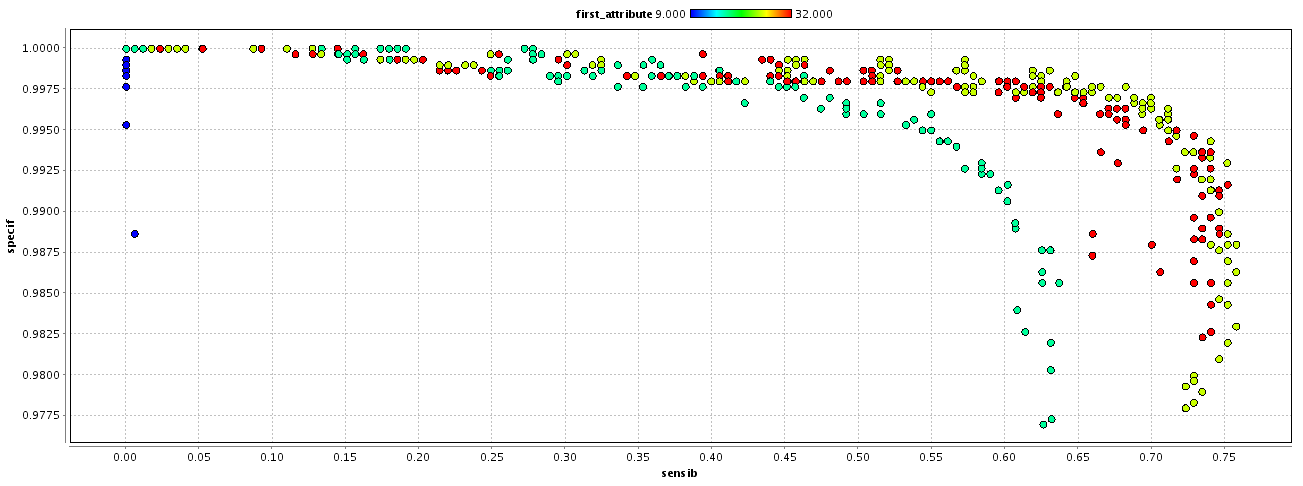
\includegraphics[width=14cm]{images/pareto_param_range.png}

{\small d) Base Normalisée -1/+1}

\vspace{0.5cm}

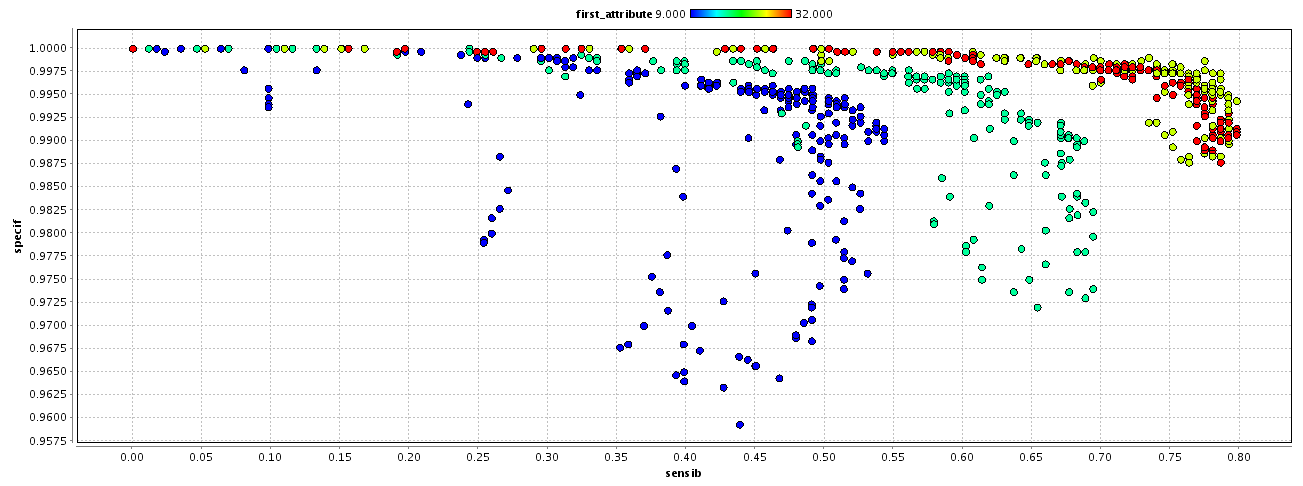
\includegraphics[width=14cm]{images/pareto_param_erosion.png}

{\small d) Base \'Erodée}


\end{center}
 \caption{Fronts de pareto des résultats de la recherche des meilleurs paramètres du classifieur (2/2). Pour chaque triplet de paramètres (C, $\gamma$, j), la sensibilité et la spécificité sont reportées sur le graphique. Le code couleur correspond à la valeur de j. En a) la base normalisation avec 200 points négatifs par image et une normalisation range. En b), la base érodée, avec 200 points négatifs par image et une normalisation \emph{moyenne}, en b) la base enrichie avec 1000 points négatifs par image et une normalisation \emph{moyenne}. }
\end{figure}




\begin{figure}[h!]
\label{fig:paramsParams}
%	\begin{center}
		\begin{tabular}{c c c c c c}
  \hline
  a	& Base Témoin 	& Base Érosion	& Base appauvrie& Base enrichie & Base normalisée \\
  \hline
 C 	& 464		& 74		& 5412		& 5412		& 10000 \\
\hline
$\gamma$& 0.0053	& 0.0094	& 0.00031	& 0.0017	& 0.052 \\
\hline
j	& 3		& 3		& 3		& 4		& 3	\\
\hline
\hline
Sensibilité& 0.75	& 0.80		& \textbf{0.82}		& 0.60		& 0.76	\\
\hline
Spécificité& 0.99	& 0.99		& 0.99		& 0.99		& 0.99 \\
\hline
Précision& 0.98		& 0.98		& 0.97		& 0.99		& 0.98 \\
\hline
 		\end{tabular}

%	\end{center}
\caption{Paramètres sélectionnés pour l'optimisation des performances. Sont indiqués pour chaque base le triplet de paramètres sélectionné ainsi que sa position sur le front de pareto.}
\end{figure}


\subsection{Base témoin}

Cette base contient des données normalisées par la méthode \emph{moyenne} avec 200 points extraits de chaque image.

\subsubsection{Meilleurs paramètres de classification}

Les paramètres du classifieur sont déterminés par une recherche grille. La performance de chaque triplet (C, $\gamma$, j) est estimée en réalisant une cross-validation à 5 validations sur l'ensemble de la base d'apprentissage.
Les paramètres sont choisis à partir du front de pareto figure \ref{fig:paretoParams1}.a en maximisant la sensibilité.


\subsection{Base Érosion}

Cette base contient des données normalisées par la méthode \emph{moyenne} avec 200 points extraits de chaque image érodée (2 voxels).


\subsection{Base Appauvrie}

Cette base contient des données normalisées par la méthode \emph{moyenne} avec 100 points extraits de chaque image.


\subsection{Base Enrichie}

Cette base contient des données normalisées par la méthode \emph{moyenne} avec 1000 points extraits de chaque image.



\subsection{Base Normalisation}

Cette base contient des données normalisées par la méthode range avec 200 points extraits de chaque image.


\subsection{Courbe Free-ROC}

Voir figure \ref{lab:froc_comp_static}
Le maximum de performances est apporté par la combinaison de 200 points avec mean/std.

\begin{figure}[h!]
 
 \begin{center}
   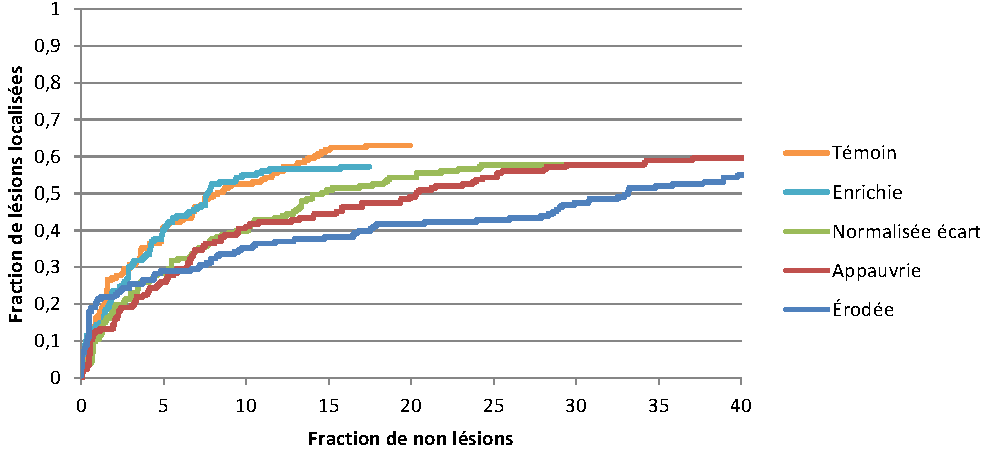
\includegraphics[width=15cm]{images/FROC_param}
 \end{center}
 \caption{\label{lab:froc_comp_static} Courbe Free-ROC comparant les performances du CAD sur une base témoin (normalisation \emph{moyenne} et 200 points négatifs par image), sur une base enrichie (1000 points négatifs par image), sur une base appauvrie (100 points négatifs par image), sur une base normalisée différemment (normalisation entre -1 et +1 et 200 points négatifs par image) et enfin sur une base de 100 points négatifs par image mais dont les volumes ont été érodés de 2 voxels.}

\end{figure}


\subsection{Comparaison des performances JAFROC}

La p-value est de 0.049, ce qui permet pas déclarer que au moins deux paramètres testés sont différents. \ref{lab:fom_param}


\begin{figure}[h!]
 \begin{center}
   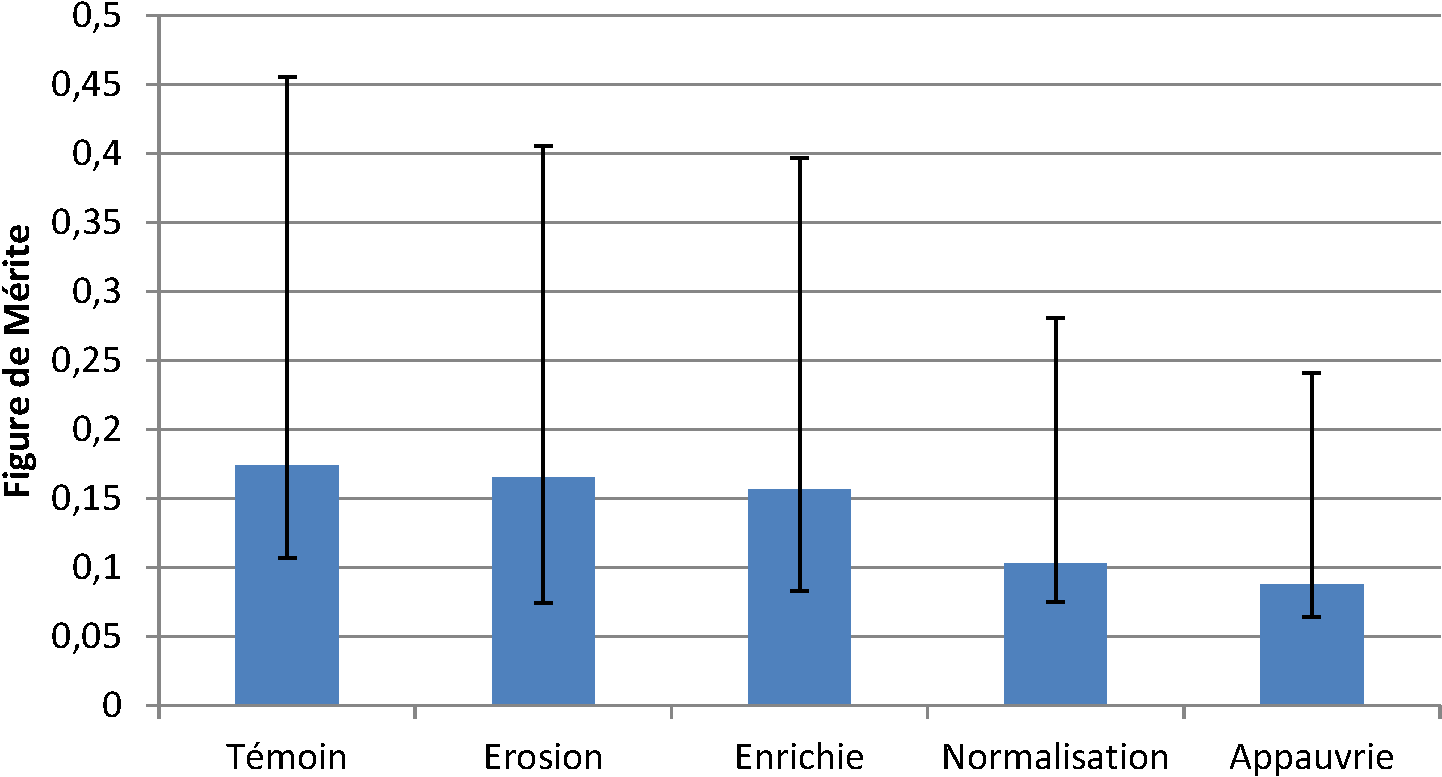
\includegraphics[width=15cm]{images/FOM_param}
 \end{center}
 \caption{ \label{lab:fom_param} Les FOM (Figure de Mérite) obtenues pour les différents paramètres}
\end{figure}

\FloatBarrier

\section{Comparaison des performances des différentes méthodes Poumon}

Les caractéristiques utilisées pour obtenir ces résultats sont les suivants :

\begin{itemize}
 \item 200 points tirés aléatoirement dans le volume de chaque image (hors tumeurs)
 \item normalisation par moyennage et neutralisation de la variance 
\end{itemize}


\begin{figure}[h!]

\begin{center}
 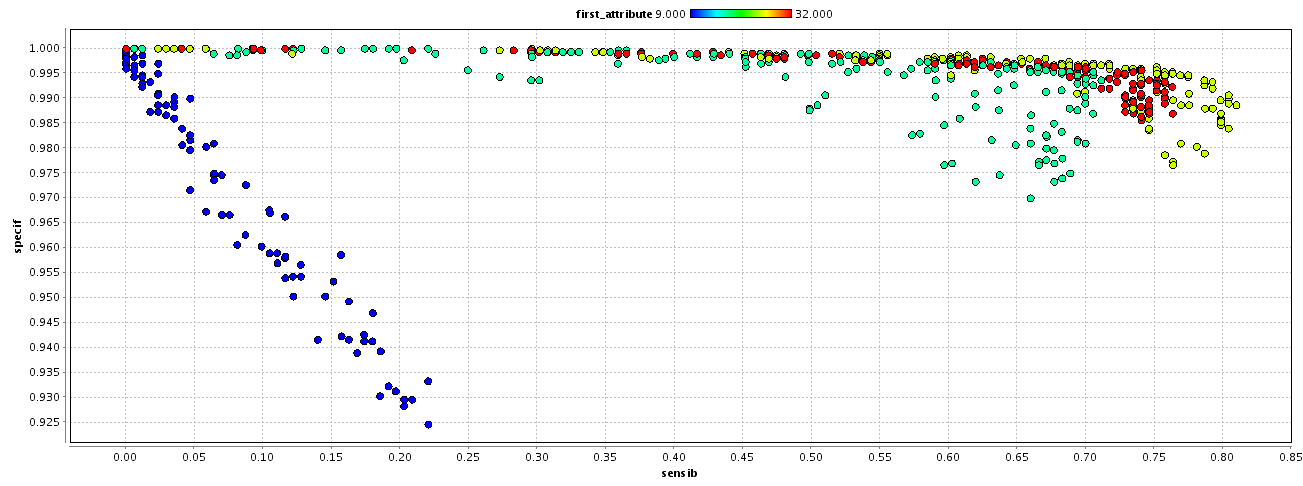
\includegraphics[width=14cm]{images/pareto_mod_IM.png}

{\small a) ET-IM}
\vspace{0.5cm}

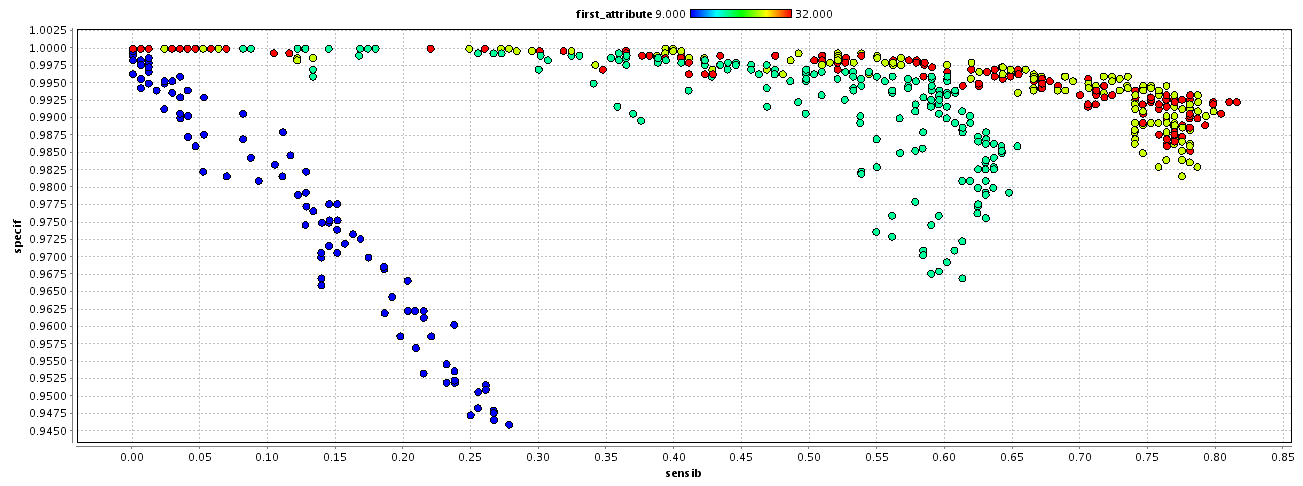
\includegraphics[width=14cm]{images/pareto_mod_LOR.png}
 
{\small b) ET-LOR}
\vspace{0.5cm}

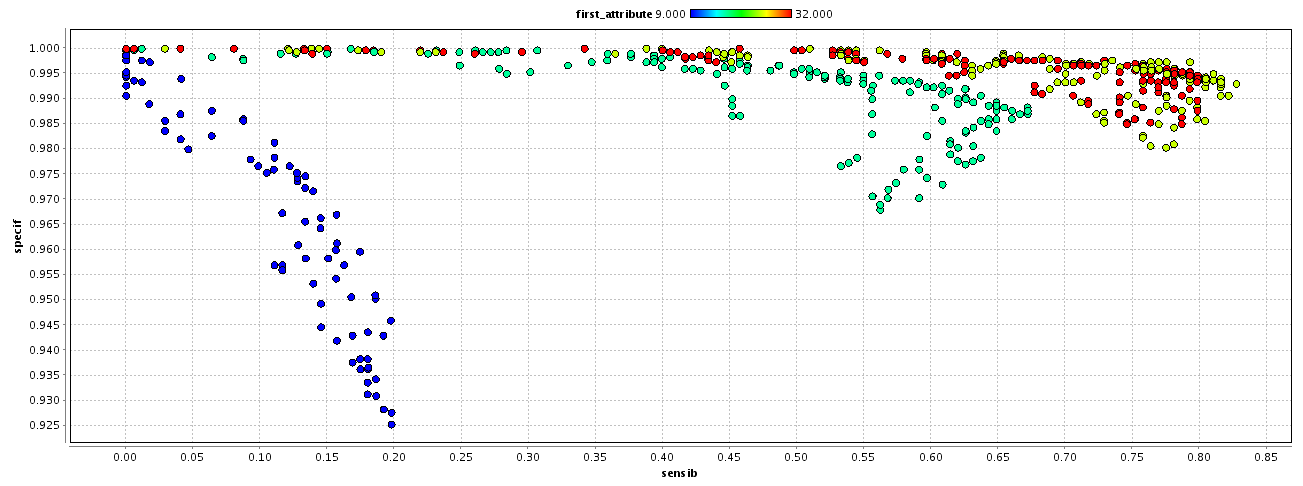
\includegraphics[width=14cm]{images/pareto_mod_NoCorr.png}

{\small c) ET-NoCorr}

\end{center}
 \caption{\label{fig:paretoModalite} Fronts de pareto des résultats de la recherche des meilleurs paramètres du classifieur pour les différentes modalités, avec 200 points négatifs par image. Pour chaque triplet de paramètres (C, $\gamma$, j), la sensibilité et la spécificité sont reportées sur le graphique. Le code couleur correspond à la valeur de j. a) représente la correction d'image ET-IM, b) les images non corrigées du mouvement, et c) les images corrigées par la méthode LOR.}
\end{figure}








\begin{figure}[h!]
\label{fig:paramsModPoumon}
%	\begin{center}
		\begin{tabular}{c| c c c c c}
  \hline
  a	& Base Statique	& Base IM	& Base LOR	& Base NoCorr	\\
  \hline
 C 	& 464		& 10000		& 10000		& 10000		\\
\hline
$\gamma$& 0.0053	& 0.00097	& 0.00031	& 0.00055	\\
\hline
j	& 3		& 3		& 4		& 3		\\
\hline
\hline
Sensibilité& 0.75	& 0.81		& 0.82		& 0.83	\\
\hline
Spécificité& 0.99	& 0.99		& 0.99		& 0.99		\\
\hline
Précision& 0.98		& 0.98		& 0.98		& 0.98		\\
\hline
 		\end{tabular}

%	\end{center}
\caption{Paramètres sélectionnés pour l'optimisation des performances du Poumon. Sont indiqués pour chaque base le triplet de paramètres sélectionné ainsi que sa position sur le front de pareto.}
\end{figure}



\subsection{ET-IM}

Cette base contient des données normalisées par la méthode mean/std. avec 200 points extraits de chaque image.




\subsection{ET-LOR}

Cette base contient des données normalisées par la méthode mean/std. avec 200 points extraits de chaque image.


\subsection{ET-NoCorr}

Cette base contient des données normalisées par la méthode mean/std. avec 200 points extraits de chaque image.


\subsection{Comparaison des performances JAFROC}

La p-value est de 0.10, ce qui ne permet pas de déclarer que statistiquement les données sont différentes : \ref{lab:fom_mod19}.

\begin{figure}[h!]
 \begin{center}
   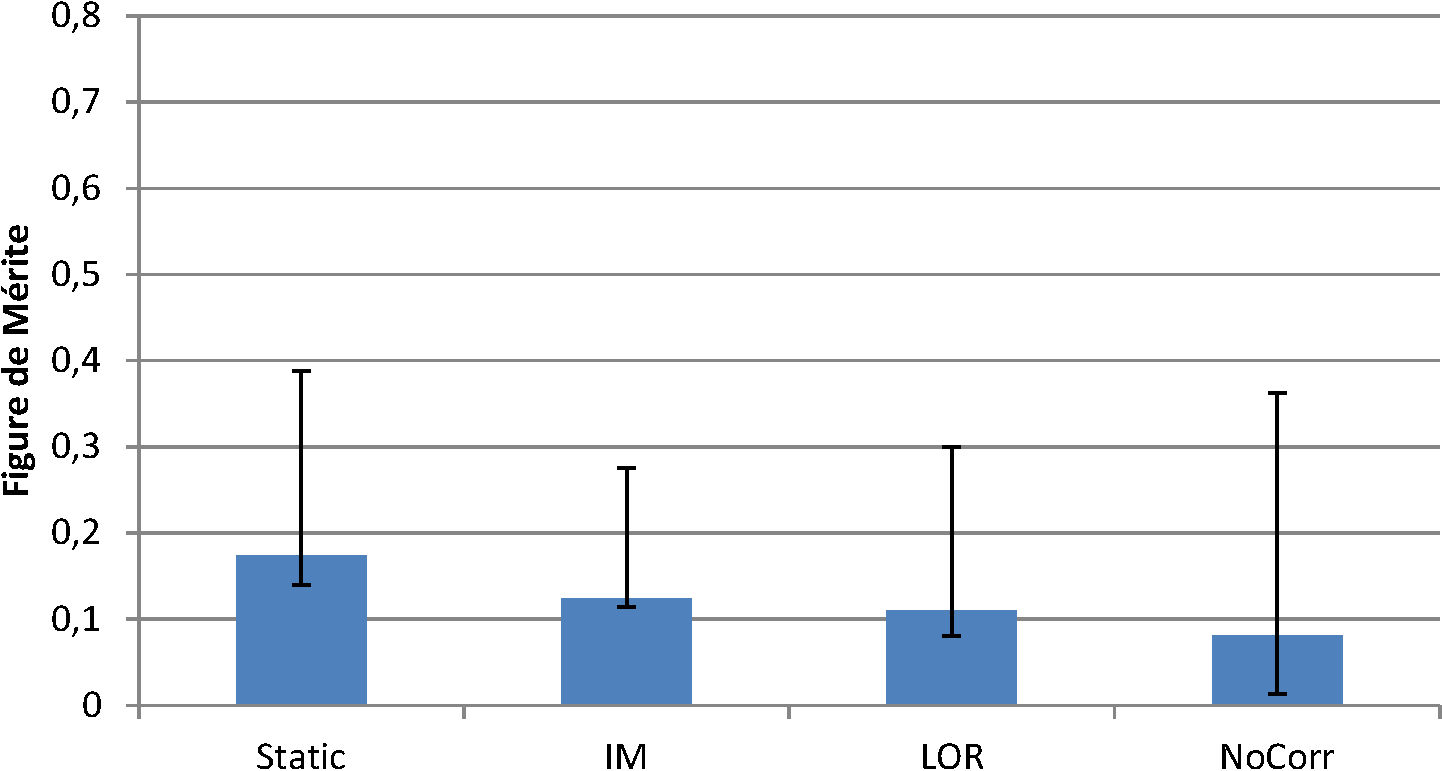
\includegraphics[width=15cm]{images/FOM_mod}
 \end{center}
 \caption{ \label{lab:fom_mod19} Les FOM (Figure de Mérite) obtenues pour les différentes modalités.}
\end{figure}

\subsection{Courbes Free-ROC}

Voir figure \ref{lab:froc_mod}.
Le maximum de performances est apporté par les images statiques, suivi par les images ET-IM.

\begin{figure}[h!]
 \begin{center}
   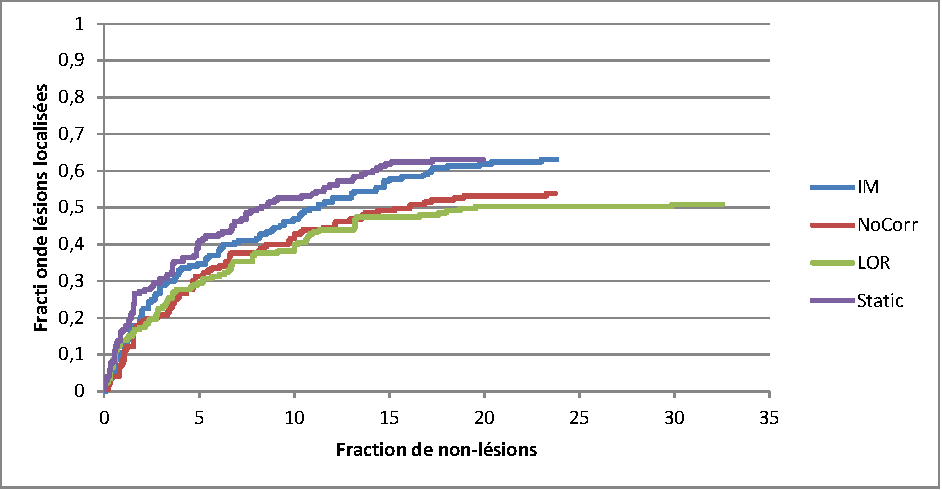
\includegraphics[width=15cm]{images/FROC_mod}
 \end{center}
 \caption{ \label{lab:froc_mod} Courbe Free-ROC comparant les performances du CAD selon les modalités de correction du mouvement respiratoire.}
\end{figure}


\FloatBarrier

\section{Comparaison des performances des différentes méthodes Foie}

Les caractéristiques utilisées pour obtenir ces résultats sont les suivants :

\begin{itemize}
 \item 200 points tirés aléatoirement dans le volume de chaque image (hors tumeurs)
 \item normalisation par moyennage et neutralisation de la variance 
\end{itemize}

\subsection{Comparaison des performances JAFROC}

La p-value est de 0.1, ce qui ne permet pas de déclarer que statistiquement les données sont différentes : \ref{lab:fom_mod19}


\begin{figure}[h!]
 \begin{center}
   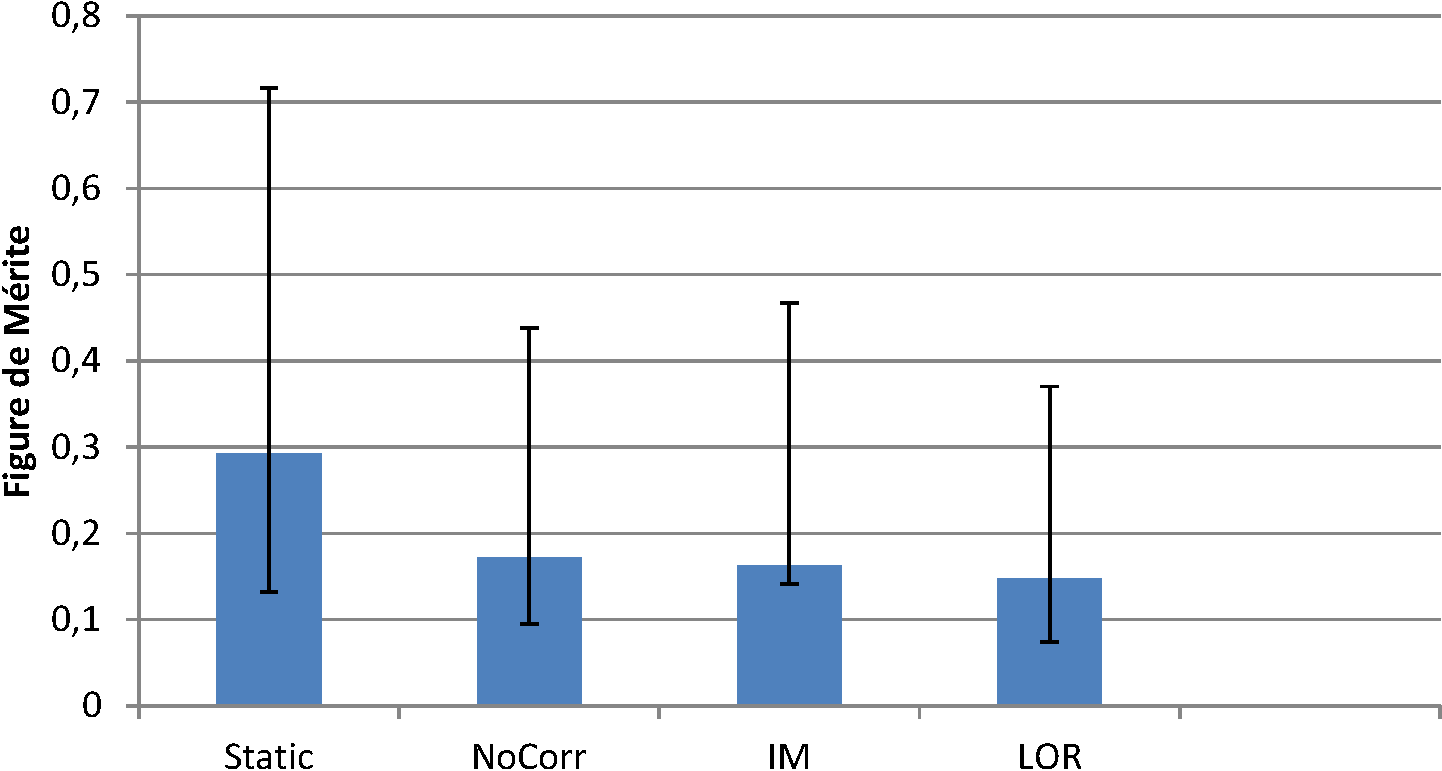
\includegraphics[width=15cm]{images/FOM_mod19}
 \end{center}
 \caption{ \label{lab:fom_mod19} Les FOM (Figure de Mérite) obtenues pour les différentes modalités.}
\end{figure}


\subsection{Courbes Free-ROC}

Voir figure \ref{lab:froc_mod19}.
Le maximum de performances est apporté par les images statiques, suivi par les images ET-IM.

\begin{figure}[h!]
 \begin{center}
   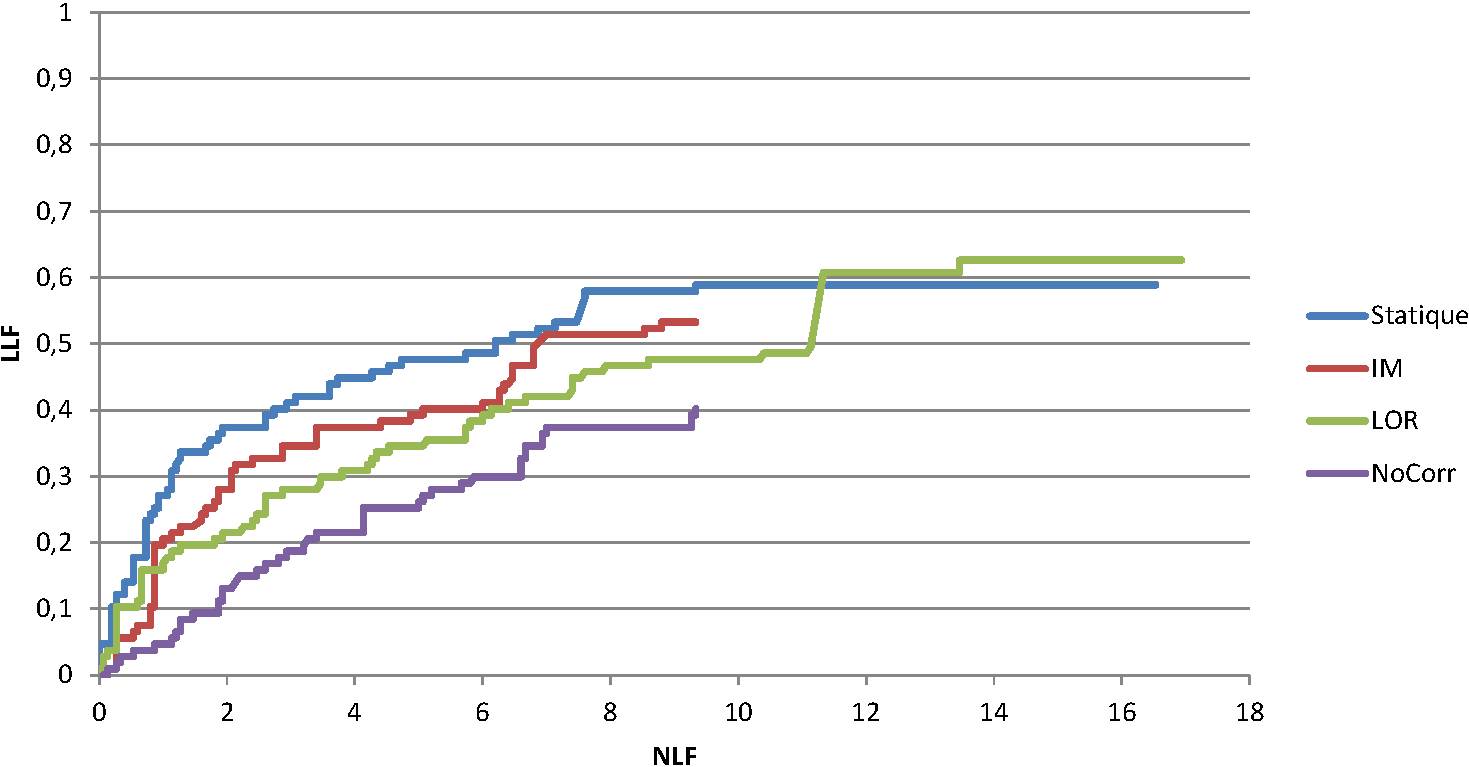
\includegraphics[width=15cm]{images/FROC_mod19}
 \end{center}
 \caption{ \label{lab:froc_mod19} Courbe Free-ROC comparant les performances du CAD selon les modalités de correction du mouvement respiratoire.}
\end{figure}


\begin{figure}[h!]

\begin{center}
 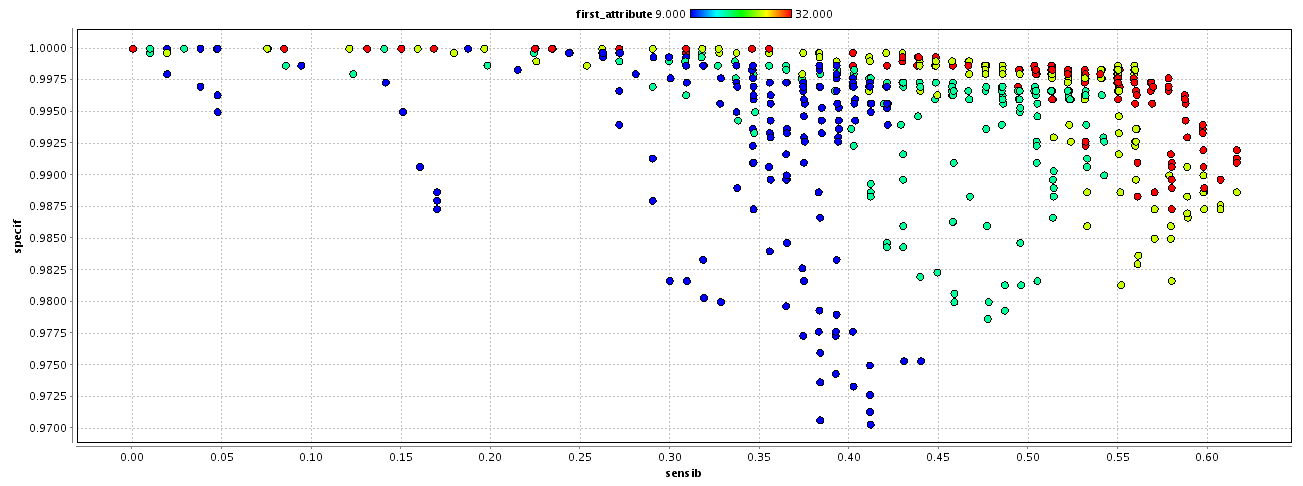
\includegraphics[width=14cm]{images/pareto_mod_Static19.png}

{\small a) ET-Static}
\vspace{0.5cm}

 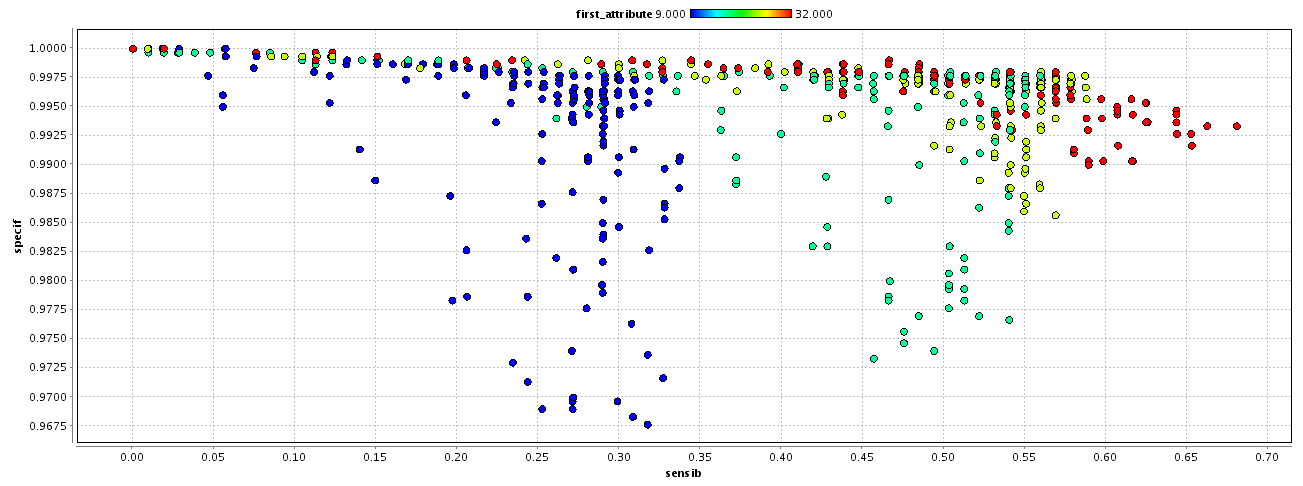
\includegraphics[width=14cm]{images/pareto_mod_IM19.png}

{\small b) ET-IM}

\end{center}
 \caption{\label{fig:paretoModalite19_1} Fronts de pareto des résultats de la recherche des meilleurs paramètres du classifieur pour les différentes modalités, avec 200 points négatifs par image. Pour chaque triplet de paramètres (C, $\gamma$, j), la sensibilité et la spécificité sont reportées sur le graphique. Le code couleur correspond à la valeur de j. a) représente la correction d'image ET-Static, b) les images corrigées du mouvement post-reconstruction.}
\end{figure}

\begin{figure}[h!]

\begin{center}
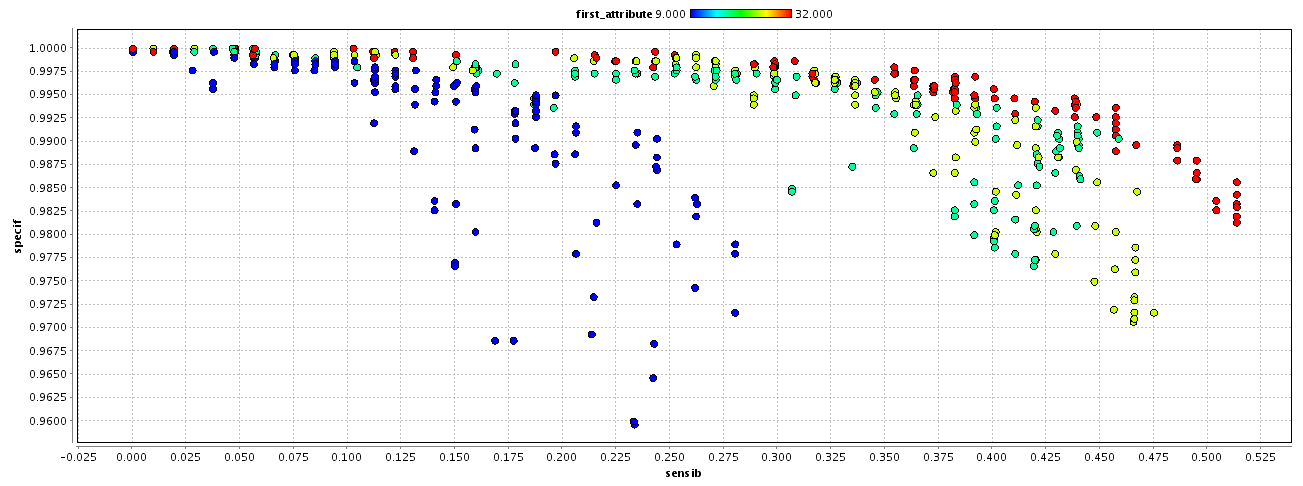
\includegraphics[width=14cm]{images/pareto_mod_LOR19.png}
 
{\small c) ET-LOR}
\vspace{0.5cm}

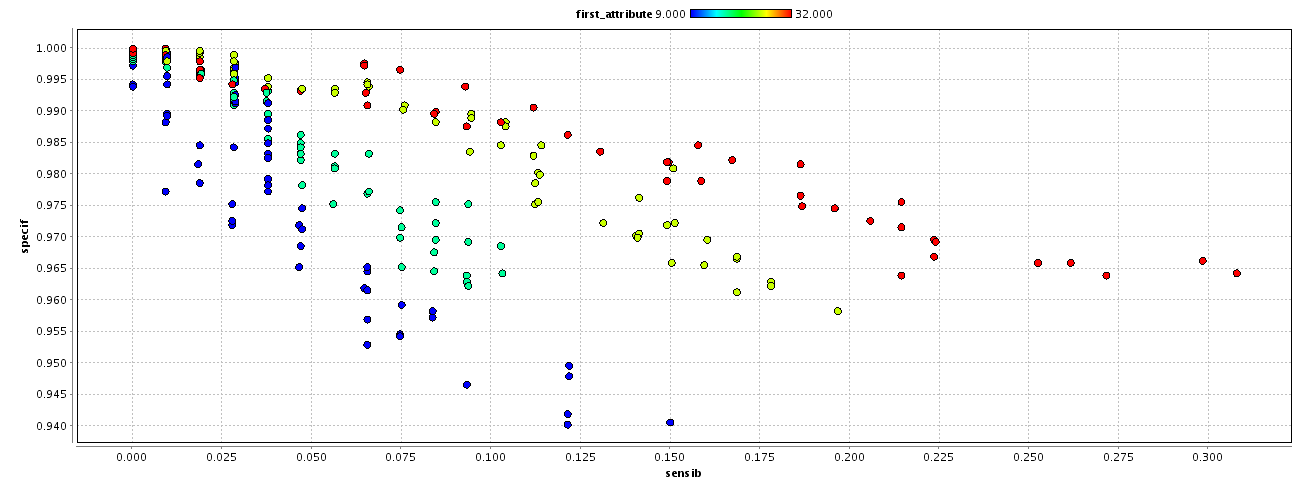
\includegraphics[width=14cm]{images/pareto_mod_NoCorr19.png}

{\small d) ET-NoCorr}

\end{center}
 \caption{\label{fig:paretoModalite19_2} Fronts de pareto des résultats de la recherche des meilleurs paramètres du classifieur pour les différentes modalités, avec 200 points négatifs par image. Pour chaque triplet de paramètres (C, $\gamma$, j), la sensibilité et la spécificité sont reportées sur le graphique. Le code couleur correspond à la valeur de j. c) représente la correction d'image pendant la reconstruction et d) le images non corrigées.}
\end{figure}



% Static : 857.6958985908936	0.001709975946676697	32.0	0.9790779315594078	0.6160173160173159	0.992
% LOR	 : 251.18864315095797	0.005323362023203629	32.0	0.969422309209811	0.5134199134199134	0.9856666666666667 
% NoCorr : 5411.6952654646375	0.001709975946676697	32.0	0.9417478291936561	0.30779220779220784	0.9643333333333333
% IM	 : 5411.6952654646375	5.49280271653059E-4	32.0	0.9826195691007659	0.6805194805194804	0.9933333333333334
\begin{figure}[h!]
\label{fig:paramsModFoie}
%	\begin{center}
		\begin{tabular}{c| c c c c c}
  \hline
  a	& Base Statique	& Base IM	& Base LOR	& Base NoCorr	\\
  \hline
 C 	& 858		& 5412		& 251		& 5412		\\
\hline
$\gamma$& 0.002		& 0.00055	& 0.0053	& 0.0017	\\
\hline
j	& 4		& 4		& 4		& 4		\\
\hline
\hline
Sensibilité& 0.62	& 0.68		& 0.51		& 0.31	\\
\hline
Spécificité& 0.99	& 0.99		& 0.99		& 0.96		\\
\hline
Précision& 0.98		& 0.98		& 0.97		& 0.94		\\
\hline
 		\end{tabular}

%	\end{center}
\caption{Paramètres sélectionnés pour l'optimisation des performances du Foie. Sont indiqués pour chaque base le triplet de paramètres sélectionné ainsi que sa position sur le front de pareto.}
\end{figure}
